\def\DevnagVersion{2.15}\documentclass[12pt]{article}
\usepackage{devanagari}
\usepackage{cite}
\usepackage{pstricks}
\usepackage{pst-node}
\usepackage{pst-coil}
\usepackage{pst-rel-points}
\usepackage{graphics}
\usepackage{epsfig}
\usepackage{verbatim, hyperref, color}
\usepackage{float}
\usepackage[margin=3cm]{geometry}
\usepackage[T1]{fontenc}
\usepackage[english]{babel}
\setlength{\parindent}{0pt}
\setlength{\parskip}{0.2cm}
\topskip 0.0in

\title{Interpreter for Geometric Constructions}
\author{Jeetesh Mangwani \& Pankaj Prateek\\
	Advisor: Dr. Amitabh Mukherjee\\
        Dept. of Computer Science and Engineering\\
	Indian Institute of Technology, Kanpur, India\\
	\{jeeteshm, pratikkr, amit\} @ cse.iitk.ac.in}
\date{November 14, 2013}

\begin{document}
\maketitle
\begin{center}{\b \em ABSTRACT}\end{center}
{\em In this project, we take up the problem of designing and implementing a language-independent interpreter for drawing geometric diagrams, focusing mainly on ruler and compass based construction problems. We start with the use cases and motivations on why such a system would be useful and what places deploying it would be fruitful. We give a brief tabulated summary review of related research work done on geometry related problems and point out the common trait that they lack the ability to decipher any problem/constraint expressed in a natural language. We, then, move to describing the design of the interpreter and the usage of cross-lingual technique to provide language-independent interpretation ability. We briefly mention how is the alignment model exploited to realize the powerful translation feature. This is followed by accounts about the work done during this semester, results obtained, difficulties faced and plan for the next semester.}

\section{Objective}
To design and implement interpreter that
\begin{itemize}
	\item is language-independent (works for English, Hindi at present)
	\item Receives steps for a geometric construction as input e.g. "Draw a line segment AB of length 4 cm", "{\dn k\?{\qva}\qb{d}} B {\dn aOr E/>yA} 5 {\dn s\?mF l\?kr ek cAp KF{\qva}Ece jo phl\? KF{\qva}cF cAp ko} C {\dn pr kAVtA ho}" etc
	\item Outputs the geometric figure obtained on executing the given sequence of steps 
\end{itemize}

\section{Introduction}
It is often the case that students, teachers, architects and artists need to draw complex diagrams manually using simple geometric instruments like ruler, compass, set squares, dividers etc. This demands labor, time as well as expertise. Resorting to sophisticated graphics applications requires knowhow of application-specific details as well as expertise in coordinating hand micro-movements.\\

In order to save these resources required in drawing geometric diagrams as well as to reduce dependence on complex graphics applications, this project introduces an interpreter for diagram construction steps expressed in a suitable natural language. This not only simplifies the construction, but also leads to easily understood natural language `programs'.\\

\section{Related work}
One of the most common techniques today to perform effective parsing is to use Part-of-Speech tagged language banks. Only few languages (about 8-10 of the 600+ languages in wide use) have the privilege of being resource-rich in the sense of having Penn-tree banks and other large-sized standardised corpus. An important observation is that fixed grammars, POS tags etc used in traditional parsers are not always the best way to break up a language. Taking a note of these shortcomings, we take a statistical approach to learn a language.\\

There has been a significant amount of work done on solving geometry construction problems. Gulwani et. al. \cite{gulwani2011synthesizing} propose a method that uses goal-based heuristic to simulate backward deduction to solve a problem expressed in a predefined logical construct. Schreck et. al. \cite{schreck2012geometric} talk about the same problem but use CAD methods to deal with constraints. At the same time, Itzhaky et. al. \cite{itzhaky2012solving} use the number of nondeterministic choices as a measure of a good solution. Ahmed, Umair et. al. \cite{ahmed2012can} look more into using domain-specific measures to minimize parser errors and augment the geometry problem solver, GeoSynth. All these papers have provided us with valuable insights into selecting important and expressive constructs for our intermediate language.



We summarize our observations in terms of following 3 parameters:
\begin{itemize}
\item Uses other linguistic/domain knowledge
\item Assumes linguistic cues are already translated into logical forms
\item Uses Parse knowledge
\end{itemize}

\begin{table}[H]
\smallskip
\begin{center}
\begin{tabular}{p{0.35\textwidth}p{0.20\textwidth}p{0.20\textwidth}p{0.20\textwidth}}
\hline
\bf{\small Paper} & \bf{\small Uses other linguistic/domain knowledge} & \bf{\small Assumes linguistic clues already traslated into logical forms} & \bf{\small Uses parse knowledge}\\[0.2cm]\hline
Geometric Construction Problem Solving in Computer-Aided Learning\cite{schreck2012geometric} & \texttt{YES} & \texttt{YES} & \texttt{NA}\\\\
Synthesizing geometry constructions\cite{gulwani2011synthesizing} & \texttt{YES} & \texttt{YES} & \texttt{NA}\\\\
Solving geometry problems using a combination of symbolic and numerical reasoning\cite{itzhaky2012solving} & \texttt{YES} & \texttt{YES} & \texttt{NA}\\\\
Can modern statistical parsers lead to better natural language understanding for education?\cite{ahmed2012can} & \texttt{YES} & \texttt{NO} & \texttt{YES}\\\\
Learning to map sentences to logical form: Structured classification with probabilistic categorial grammars\cite{zettlemoyer2012learning} & \texttt{YES} & \texttt{NO} & \texttt{YES}\\
\hline
\end{tabular}
\caption{Related Works}
\end{center}
\end{table}

Unlike all previous attempts, we do not assume that the logical forms of the sentences are available, nor we assume the availability of a parser. We use cross-lingual alignment to map the given sentence in natural language to metalanguage. It is therefore applicable to a large range of languages. We demonstrate this for two widely known languages belonging to very different families - Hindi and English.


% \subsection{Learning to map sentences to logical form: Structured classification with probabilistic categorical grammars\cite{zettlemoyer2012learning}}
% 
% \subsection{Geometric Construction Problem Solving in Computer-Aided Learning\cite{schreck2012geometric}}
% 
% \subsection{Synthesizing geometry constructions\cite{gulwani2011synthesizing}}
% 
% \subsection{Can modern statistical parsers lead to better natural language understanding for education?\cite{ahmed2012can}}
% 
% \subsection{Solving geometry problems using a combination of symbolic and numerical reasoning\cite{itzhaky2012solving}}

\section{Design}
The interpreter consists of two main components:
\begin{itemize}
\item Aligner
\item Metalanguage Interpreter
\end{itemize}

\subsection{Aligner}
Cross-lingual alignment is the heart of the learning mechanism in this project. It is used to obtain mapping/alignment between a natural language and our carefully designed and structured imperative metalanguage, L0. Since this alignment can be obtained for any natural language, the application is scalable to any number of natural languages.\\

We have used GIZA++ \cite{och2003systematic} as the cross-lingual aligner. GIZA++ is a statical machine translation toolkit that is used to train IBM Models 1-5 and an HMM word alignment model.\\

\subsection{Metalanguage Interpreter}
The interpreter component exploits the alignment model obtained from the Aligner component. Given a sentence expressed in a natural language, we use the alignment model to get statistically most probable interpretation in L0. A command in L0 is then used to output the desired figure.

\section{Cross-Lingual alignment}
Cross-Lingual alignment is a technique to statistically align the words of a given pair of languages. It is close to translating one language into another, without any syntactic or semantic knowledge of any of the languages. As an example, for a pair of langauges, given sufficiently many sentences as illustrated in the table 2, a cross-lingual alignment assigns probabilities to the event that a particular source-language token is mapped to a target-language token.\\

\begin{table}[H]
\smallskip
\begin{center}
\begin{tabular}{p{0.33\textwidth}p{0.33\textwidth}p{0.33\textwidth}}
\hline
\vspace{0.1cm}\bf{English} & \vspace{0.1cm}\bf{Hindi} & \vspace{0.1cm}\bf{Meta Language}\\[0.2cm]\hline
Construct a line AB of length 4 cm & 4 {\dn s\?mF lMbAI kA ek r\?KAK\317wX} AB {\dn KF{\qva}Ece} & \texttt{construct lineSegment AB length 4 cm}\\[0.2cm]
With A as center and radius 3 cm, draw an arc & {\dn k\?{\qva}\qb{d}} A {\dn aOr E/>yA} 3 {\dn s\?mF l\?kr ek cAp KF{\qva}Ece} & \texttt{constrcut arc center A radius 3 cm}\\[0.2cm]
With B as center and radius 5 cm, draw an arc cutting the previously drawn arc at C & {\dn k\?{\qva}\qb{d}} B {\dn aOr E/>yA} 5 {\dn s\?mF l\?kr ek cAp KF{\qva}Ece jo phl\? KF{\qva}cF cAp ko} C {\dn kAVtA ho} & \texttt{construct intersectingArc center C radius 5 cm cuts arc previous at C}\\[0.2cm]
\hline
\end{tabular}
\caption{Sample Corpus}
\end{center}
\end{table}

\begin{table}[H]
\smallskip
\begin{center}
\begin{tabular}{p{0.33\textwidth}p{0.33\textwidth}c}
\hline
\bf{English} & \bf{Meta Language} & \bf{Probability}\\[0.2cm]\hline
Construct & \texttt{construct} & 1.00\\
Line segment & \texttt{lineSegment} & 1.00\\
intersects & \texttt{intersect} & 0.93\\
intersect eachother & \texttt{intersect} & 0.78\\
cut eachother & \texttt{intersect} & 0.87\\
cut & \texttt{cut} & 0.98\\
join & \texttt{join} & 1.00\\
mark & \texttt{mark} & 0.98\\
label & \texttt{mark} & 0.98\\
bisector & \texttt{bisector} & 0.60\\
interior & \texttt{interior} & 0.20\\
exterior & \texttt{exterior} & 0.20\\
\hline
\end{tabular}
\caption{Sample alignment between English and Metalanguage}
\end{center}
\end{table}

\begin{table}[H]
\smallskip
\begin{center}
\begin{tabular}{p{0.25\textwidth}p{0.25\textwidth}c}
\hline
\bf{Hindi} & \bf{Meta Language} & \bf{Probability}\\[0.2cm]\hline
{\dn lgA dFEjy\?} & \texttt{construct} & 0.90\\
{\dn KF{\qva}Ece} & \texttt{construct} & 0.98\\
{\dn rcnA kFEjy\?} & \texttt{construct} & 0.96\\
{\dn bnAiy\?} & \texttt{construct} & 0.98\\
{\dn r\?KAK\317wX} & \texttt{lineSegment} & 1.00\\
{\dn pr-pr \3FEwEtQC\?d} & \texttt{intersect} & 0.98\\
{\dn kAVtA ho} & \texttt{cut} & 0.82\\
{\dn kAV\?} & \texttt{cut} & 0.95\\
{\dn EmlAiy\?} & \texttt{join} & 0.98\\
{\dn joEwy\?} & \texttt{join} & 0.98\\
{\dn a\2Ekt kFEjy\?} & \texttt{mark} & 0.98\\
{\dn mAn lFEjy\?} & \texttt{mark} & 0.98\\
{\dn smE\392wBAjk} & \texttt{bisector} & 0.59\\
{\dn a<y\306wtr} & \texttt{interior} & 0.20\\
{\dn bEhBA\0g} & \texttt{exterior} & 0.20\\
\hline
\end{tabular}
\caption{Sample alignment between Hindi and Metalanguage}
\end{center}
\end{table}

\section{What has been done}
\subsection{Corpus}
The corpus contains around 350 sentences from the geometry construction field in both the languages. These were collected from the NCERT textbooks of standards ${6^{th}}$ to ${9^{th}}$. English-to-Metalanguage and Hindi-to-Metalanguage sentence maps were generated manually which were used to train GIZA++.

This approach has been shown to work for simple construction steps. Output diagram for the steps above is shown in Figure 2.

\begin{figure}[H]
  \begin{center}
    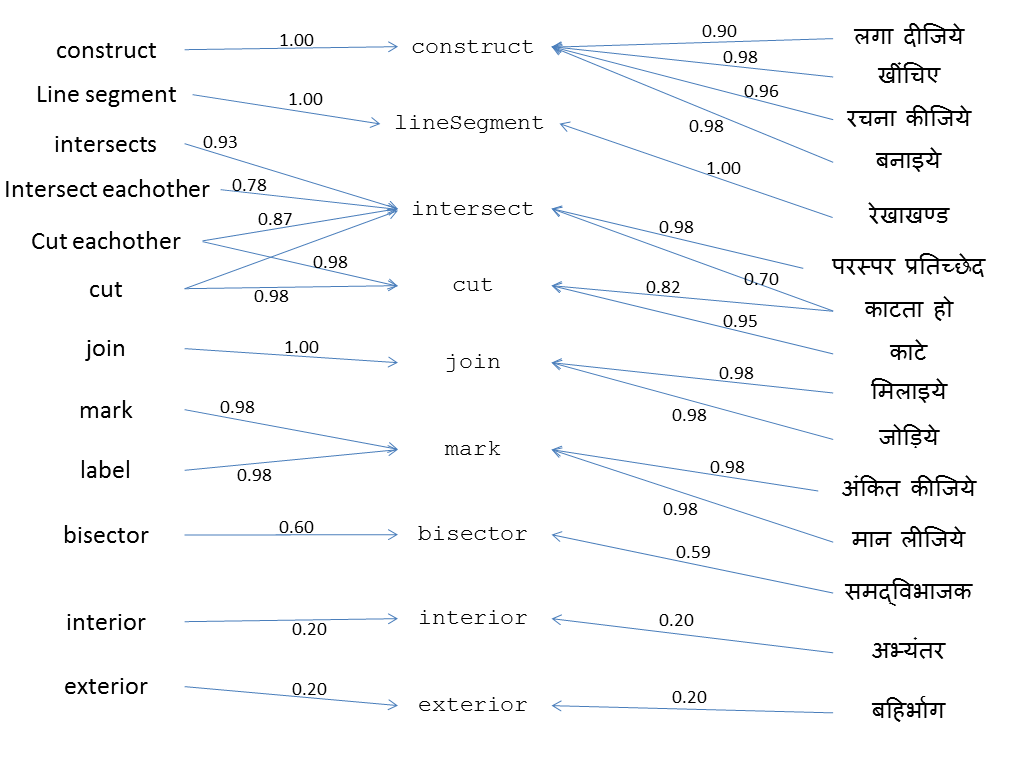
\includegraphics[scale=0.5]{image.png}
  \end{center}
  \caption{Graphical visualization of the sample alignment}
  \label{fig:pspic}
\end{figure}

% \begin{enumerate}
% \item English-to-Metalanguage and Hindi-to-Metalanguage sentence pairs have been collected from NCERT textbooks to be used in bootstrap corpus.
% \item The approach has been shown to work for simple construction steps. Output diagram for the steps above is shown in Figure 1.
\begin{figure}[H]
  \begin{center}
    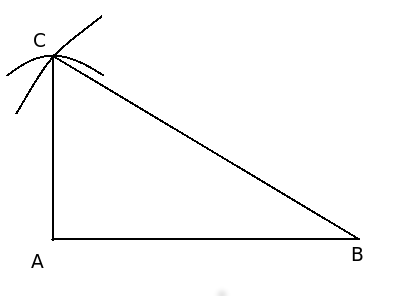
\includegraphics[scale=0.5]{triangle.png}
  \end{center}
  \caption{Constructed Triangle}
  \label{fig:pspic}
\end{figure}
%\end{enumerate}

\section{Results}
\begin{enumerate}
\item Number of sentences in the corpus: 360 each in English-to-Metalanguage and Hindi-to-Metalanguage corpus 
\item A sample prototype implementation that demonstrates the performance of the system for simple construction steps of drawing line segments and arcs.
\item Number of unique tokens in each of the three languages:\\
\begin{table}[h]
\smallskip
\begin{center}
\begin{tabular}{cc}
\hline
\bf{Language} & \bf{Number of unique tokens}\\[0.2cm]\hline
English & 181+\\
Hindi & 169+\\
Metalanguage & 110+\\
\hline
\end{tabular}
\caption{Unique tokens in different languages}
\end{center}
\end{table}
\end{enumerate}

\subsection{Difficulties}
\begin{itemize}
\item {\bf Anaphoras}
Dealing with anaphoras like ``this'', ``it'', ``previous'', ``last'' etc in sentences like ``Mark any point M on it'', ``{\dn ek \7{s}EvDAjnk E/>yA l\?kr EpCl\? crZ vAl\? cAp ko Eb\306w\7{d}} A {\dn pr kAV\?{\qva}.}'' etc
\item {\bf Underspecified Parameters}
We also need to provide for unspecified radii, lengths and anlge measures e.g. ``With A and B as centers and a suitable radius, draw two arcs interseting eachother at point C''
\item {\bf Probabilistic Mapping}
Since the mapping is statistical in nature, there might be various close alignments for the same source-language word. This forces us to resort to try out different possible alignments and look for the one that fits e.g. for the sentence ``Construct AB of length 7.8cm'', we get the following alignments with their corresponding probabilites (we assume that probabilites of word-wise alignment are independent of eachother)
\begin{table}[H]
\begin{center}
\begin{tabular}{lc}
\hline
\bf{Mapped meta-language sentence} & \bf{Probability}\\\hline
construct AB any length 7.8cm & 0.716853\\
construct AB lineSegment length 7.8cm & 0.21081\\
construct AB angle length 7.8cm & 0.0723206\\
construct AB center length 7.8cm & 1.90645e-06\\
\hline
\end{tabular}
\caption{Map to possible metalanguage sentences alongwith their probabilities}
\end{center}
\end{table}
\end{itemize}

\section{What needs to be done}
\begin{enumerate}
\item Enrich the corpus to cover larger domains of expressions e.g. having larger number of primitive steps, providing for higher-level primitives, specifying relative distances, dealing with anaphoras and references
\item Expand the functionality of the system to work for all kinds of construction steps claimed so far
\item Deploy the system on a webserver to demonstrate its functionality and work towards making it more robust
\item In order to capture colloquial (non-academic) ways of expressing construction steps, we need to develop a user interface that augments the corpus with input sentences
\end{enumerate}

\nocite{schreck2012geometric}
\nocite{gulwani2011synthesizing}
\nocite{ahmed2012can}
\nocite{itzhaky2012solving}
\nocite{zettlemoyer2012learning}
\nocite{och2003systematic}

\bibliography{report}{}
\bibliographystyle{plain-annote}
\end{document}